\documentclass{article}
\usepackage{geometry}
\geometry{ letterpaper,
 	        %total={170mm,257mm},
	        left=30mm,
	        top=30mm,}
\usepackage[utf8]{inputenc}
\usepackage{graphicx,subfigure}
\usepackage{array}
\usepackage[bookmarks=true]{hyperref}
\usepackage{bookmark,booktabs}
\usepackage{lipsum}
\usepackage{setspace}
\usepackage{datetime, hyperref, appendix}
\usepackage{amssymb,amsmath,amstext}
\usepackage{listings}
\newcommand{\duedate}{\formatdate{16}{12}{2016}}

\makeatletter % `@' now normal "letter"
\@addtoreset{equation}{section}
\makeatother  % `@' is restored as "non-letter"
\renewcommand\theequation{{\thesection}.\arabic{equation}}

% definition of a macro to produce a matrix
  \def\mtx#1#2{\renewcommand{\arraystretch}{1.0}%
      \left( \begin{array}{#1}#2\end{array} \right)}

% table/figure caption     
\renewcommand {\thetable} {\thesection{}.\arabic{table}}
\renewcommand {\thefigure} {\thesection{}.\arabic{figure}}

%\setlength{\parindent}{4em}
\setlength{\parskip}{0.5em}
\renewcommand{\baselinestretch}{1.25}

\newcommand{\forceindent}{\leavevmode{\parindent=3em\indent}}

\pagenumbering{gobble}


\begin{document}
{\setstretch{1.0}
\title{\bf Evaluation of Customer Interest-Level of \\
House Rental Listings \vspace{0.25em}}
\author{
        DS-GA 1003 Course Project \vspace{0.5em}\\
        Machine Learning and Computational Statistics  \vspace{2.0em}\\
        Xialiang Liu, Yihui Wu  \vspace{0.75em}\\
        Courant Institute of Mathematical Sciences \vspace{0.5em}\\
        New York University \\ 
\date{}
}

\maketitle
}
%\begin{abstract}
%Short introduction to subject of the paper \ldots 
%\end{abstract}
%------------------------------------------------------------- Abstract
%\begin{center}
%{\bf Abstract}
%\end{center}

%The analysis of risk--which is the total dispersion or volatility of returns for a security or portfolio--is a critical element of superior investment performance. The regression-based Multiple-Factor Model (MFM) is one of the commonly acknowledge analyzing tools for portfolio risk management. In this paper, the mathematical model of single-factor and multiple-factor regression is introduced, with applications of time series and cross-sectional regression in financial industry. This paper gives an implementation of the practical computation of portfolio risk by backtesting on Equity portfolios on historical data. The multiple-factor risk of portfolios is analyzed through comparison. Also, approach of portfolio management enlightened by the multiple-factor model is discussed. 

\pagenumbering{arabic}

%\newpage

%-------------------------------------------------------- 1. Introduction
\section{Introduction} \label{intro}

~~~ In this project, we build a predictive model about how popular an apartment rental listing is associated with the listing content. Good assessment of such listings will allow owners and agents to better understand renters' needs and preferences, and in verse make it easier for renters to find comfortable apartments.

Our objective is to give an estimation based on the available information on the rental listing websites, of the number of inquiries a listing has in the duration that the listing was live on the site, and label it with different categories.

Section \ref{setting} provides a statement of the problem and details about the dataset. Data preprocessing and selected multiclass classification algorithms are given in Section \ref{method}. Then, Section \ref{features} demonstrates the feature engineering approaches we have employed in the process of training our learning model. In Section \ref{results}, we compare the results of different algorithms and summarize the features that improving the performance of predictive model.  Further attempts is discussed in Section \ref{nextsteps}.


%----------------------------------------------------------- 2. Data Settings 
\section{Data Settings} \label{setting}

~~~~The dataset from RentHop contains 49352 listings of apartments in New York
City. The features involves multimedia data ranging from numbers, dates, categorical features, text, geographical data, and photos.
The fields of a rental listing contains are listed in Table 2.1. 

The data used in this project is available on \textit{Kaggle} as part of an ongoing competition. The data comes from \textit{renthop.com}, an apartment listing website.

\begin{table}[!htbp]
\centering
\label{datatable}
\begin{tabular}{ll}
\hline
Feature & Description \\
\hline
bathrooms & number of bathrooms \\
bedrooms & number of bathrooms \\
building\_id & the building id number with alphanumeric characters \\
created & time of the listing being available on the website \\
description & short sentences (can be empty)\\
display\_address & name of the avenue/street\\
features & a list of features/keywords about this apartment (can be empty)\\
latitude & float number representing its latitude\\
listing\_id & 7-digit number\\
longitude & float number representing its longitude\\
manager\_id & the manager id number with alphanumeric characters \\
photos & photos of apartments (provided with a link and the corresponding photos) \\
price & the price in USD \\
street\_address & detailed street information \\
\hline
\end{tabular}
\caption{Available statistics in the dataset of rental listings}\vspace{0.5em}
\end{table}

%----------------------------------------------------------- 3. Methodology
\section{Methodology} \label{method}

%----------------------------------------------- 3.1 Evaluation Metrics
\subsection{Evaluation Metrics} \label{objective}

~~~~ The level of interest is defined by the number of inquiries a listing has in the duration that the listing was live on the site, and has 3 categories: ``high'', ``medium'' and ``low''. As we will implement different algorithms to search for better solution, we need a assessment criteria for comparison. The performance of an learning model will be evaluated using the \textit{multi-class logarithmic loss}. Each listing has one true class. For each listing, we will obtain a set of predicted probabilities (one for every listing). The loss is computed as,

$$
\log loss=-1\sum_{i=1}^{N}\sum_{j=1}^{M} y_{ij}\log(p_{ij}),
$$

Besides, the prediction accuracy is another consideration in this problem. We will compare the performances of different models and evaluate the improvement of adding new features by calculating the rate of misclassifications as well.

%----------------------------------------------- 3.2 Train-test split
\subsection{Train-Test Split} \label{train_test_split}

~~~~ We separate the dataset by 50\%, 25\% and 25\%  as our training set, validation set and test set. Data samples are first grouped by classes (i.e., interest-level in this case), then do the train-test split, which guarantees that there are adequate number of samples from each class in both training set and validation/test set. 

%----------------------------------------------- 3.3 Selected Models
\subsection{Selected Models} \label{algos}


\noindent\textbf{\large Logistic Regression}

We used One-vs-Rest logistic regression as the performance benchmark. Logistic regression is known for its robustness and fast training. Empirically, with 10 data points provided for each feature, logistic regression will have a satisfactory performance. For our selection of features, except for the one hot encoding for categorical features, the numbers of features is well under 1/10 of the total data points. So we expect a reasonably good performance by logistic regression. 
% REF: van Smeden, Maarten, et al. "No rationale for 1 variable per 10 events criterion for binary logistic regression analysis." BMC Medical Research Methodology 16.1 (2016): 163
\vspace{1.5em}

\noindent\textbf{\large Random Forest}

Generally, structural risk minimization does well in binary classification with reasonable clean dataset. In a multi-class case and especially outliers are expected, a candidate of alternative algorithms is the Random Forest. The subset of training sets with bagging and subsets of features can help reduce their effect.
With randomized selection of features in the ensemble process, the correlation between trees is reduced and it is hard to overfit. 
\vspace{1.0em}

\noindent\textbf{\large AdaBoost}

AdaBoost uses weighted sum of outputs of weak learners as its final output. It is known for its resistance to overfitting. Because it uses exponential loss, it is sensitive to noisy data and outliers. Using AdaBoost algorithm will help us understand the property of our data.
\vspace{1.5em}

\noindent\textbf{\large Gradient Boosting}

We choose the Gradient Boosted Trees to improve our learning model, for it favors the features on different scale, and automatically detects (non-linear) feature interactions. In this project, we use the package of XGBoost, which is short for eXtreme Gradient Boosting package. Since XGBoost has lots of hyper-parameters, we use exhaustive grid search to find the best parameter. %While it took almost a whole night running the program, better performance certainly pays off.
\vspace{1.5em}

%--------------------------------------------------------------- 4. Features
\section{Features} \label{features}

% Start point = 5 numerical 
% 1. Adding Numerical Features
% 2. Categorical 
% 3. Non-linear Transformation on Price
% 4. Human Factor - Manager 
% 5. Clustering on Geo
% 6. tf-idf from descriptions

~~~~ We have four types of data: numerical data, categorical data, text, and photos. In our project, we will focus on processing the first three categories. Numerical features are ordered and comparable. Categorical features are categories represented with strings of alphanumerical characters. Text description is unstructured data written in natural language. Different types of processing are attempted in this project. 

Data provided by RentHop are real. So we will encounter the same situations just like searching for a listing on the Internet. It's possible that the lister provides not enough information of the listing. While price, geographical location, and created time are presented in every listing, we have different amount of missing values in other features. While some features can be estimated using mean values of existing values, some are inestimable. For example, if a listing has no text description, it's because the lister didn't provide anything and nothing itself has some information about the listing. So for this kind of features that with ``meaningful'' missing values, we keep the value missing. 

The following features are extracted as we try to improve the accuracy of prediction and the probability of predicting the correct class. 

\subsection{Adding Numerical Features}

~ A natural candidate of adding new numerical features is to describe the amount of information. Together with ``created time'' of the listings, we can extract 6 features:\vspace{1.0em}

  \texttt{\indent\textbullet ~num\_photos} = len(photo\_links)
  
  \texttt{\indent\textbullet ~num\_features} = len(data[``features''])
  
  \texttt{\indent\textbullet ~num\_description\_words} = len(data[``description''] after split) 
  
  \texttt{\indent\textbullet} ~Created month, day, and hour (3 features added)

\subsection{Categorizing Hashable Features}

~~~~ For categorical data, we tried different types of representation. First we hashed all the categories into different integers. Then, we did one-hot encoding and binary encoding for each feature.
One hot or dummy coding produces one feature per category, each of them are binary 0/1. One indicates in the category and zero the opposite. Unlike one-hot encoding, binary encoding uses the hashed integer directly in binary form and use each bit as a feature. Comparing to one hot encoding, binary encoding will have only $\log(n)$ new categorical features created instead of $n$. So the dimension is compressed.

\subsection{Non-linear Transformation on Price}

~~~~ A listing with extremely low or high price is very unlikely to attract the interests from customer. We have incorporate an non-linear transformation on ``price'' as a complement, which is orthogonal to the log price. 

Shown in Figure 4.1, we can see that the apartments with prices lower than the average price, but not in the lowest subset of prices, received the minimum score of non-linear price. 
\begin{align*}
&\text{price}_{cube} = (\text{log\_price})^3 \\
&\text{price}_{nl} = \text{price}_{cube} - \frac{<\text{price}_{cube}, ~\text{log\_price}>}{<\text{log\_price}, ~\text{log\_price}>}
\end{align*}

\begin{figure}[h]
\centering
\subfigure[Illustration of Non-linear Transformation]{
	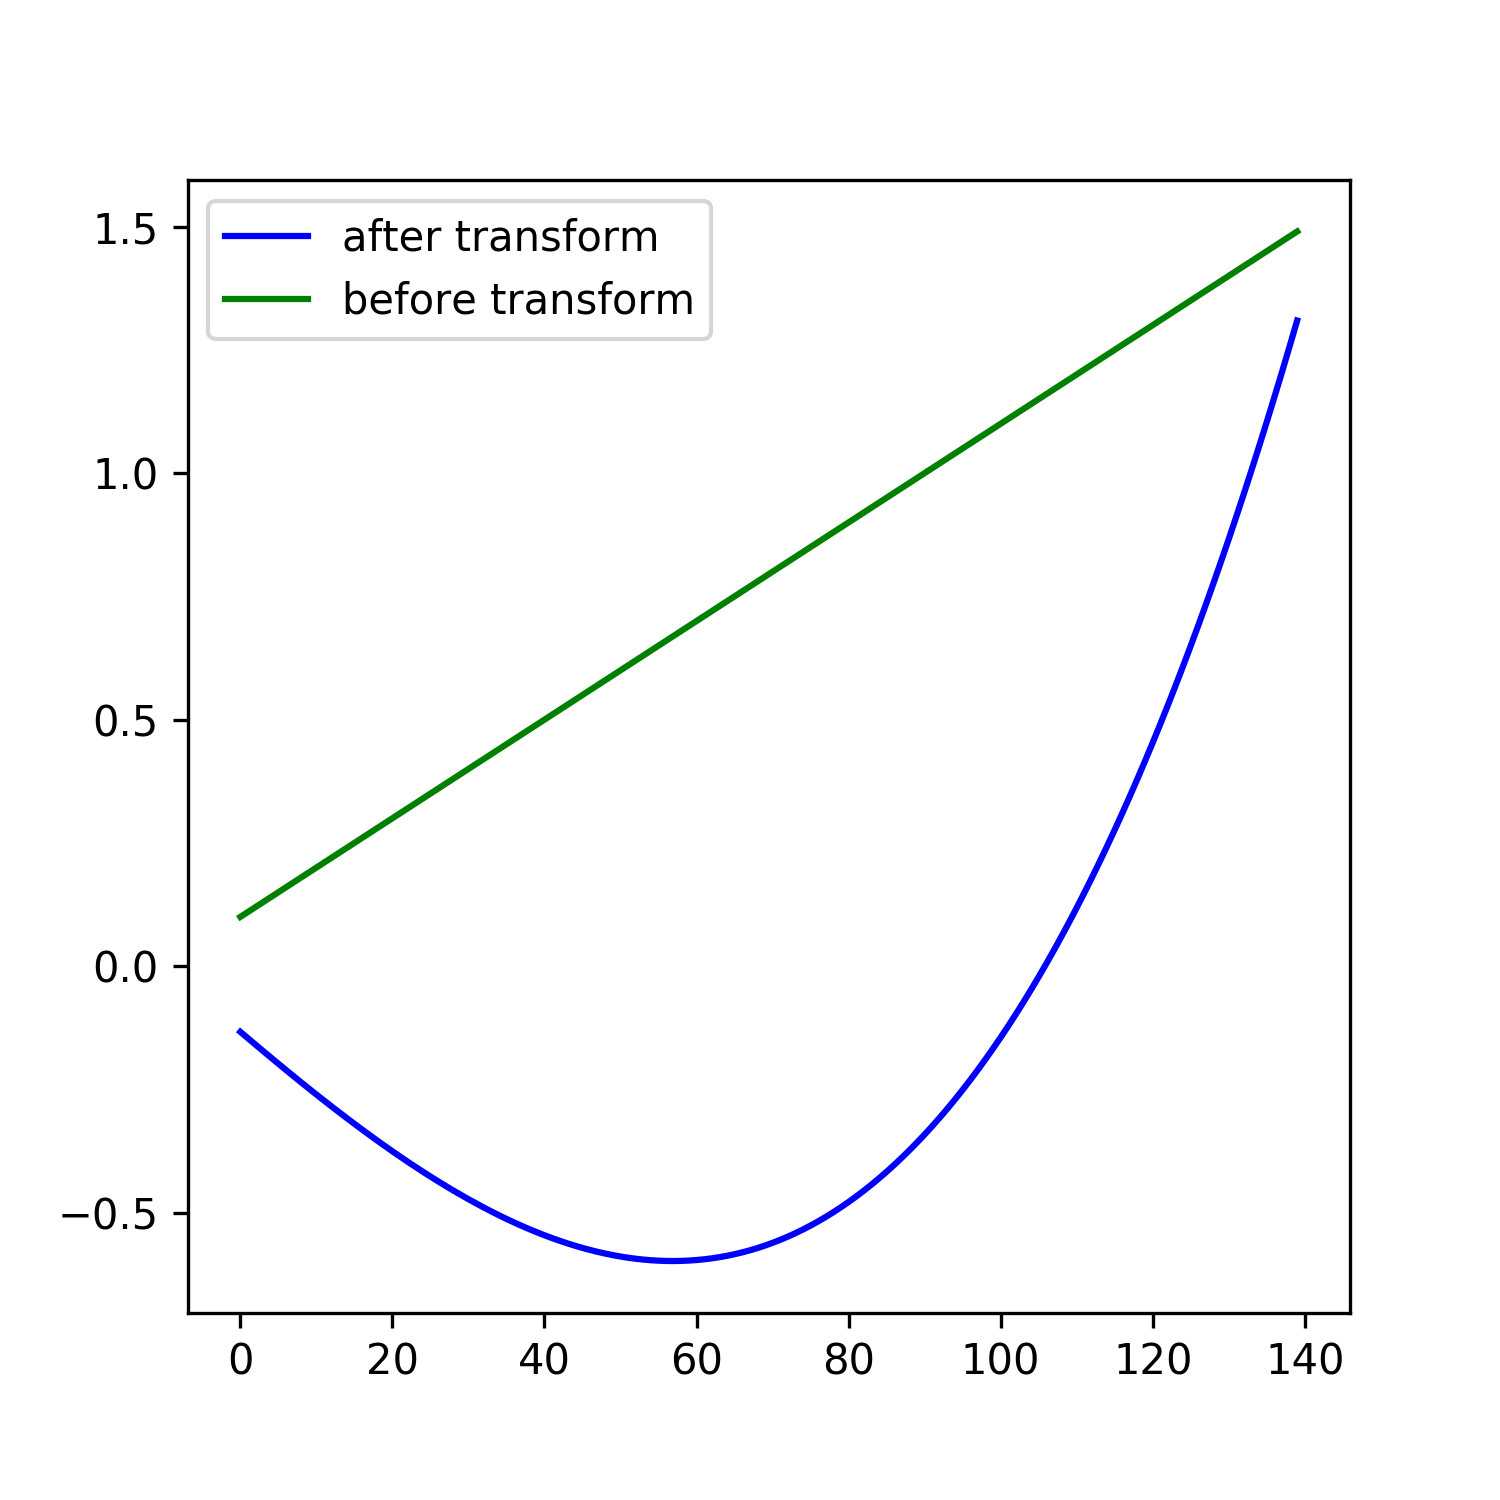
\includegraphics[width=0.3\textwidth]{pic/nonlinear_relation.png}
}
\subfigure[Non-linear Price]{
	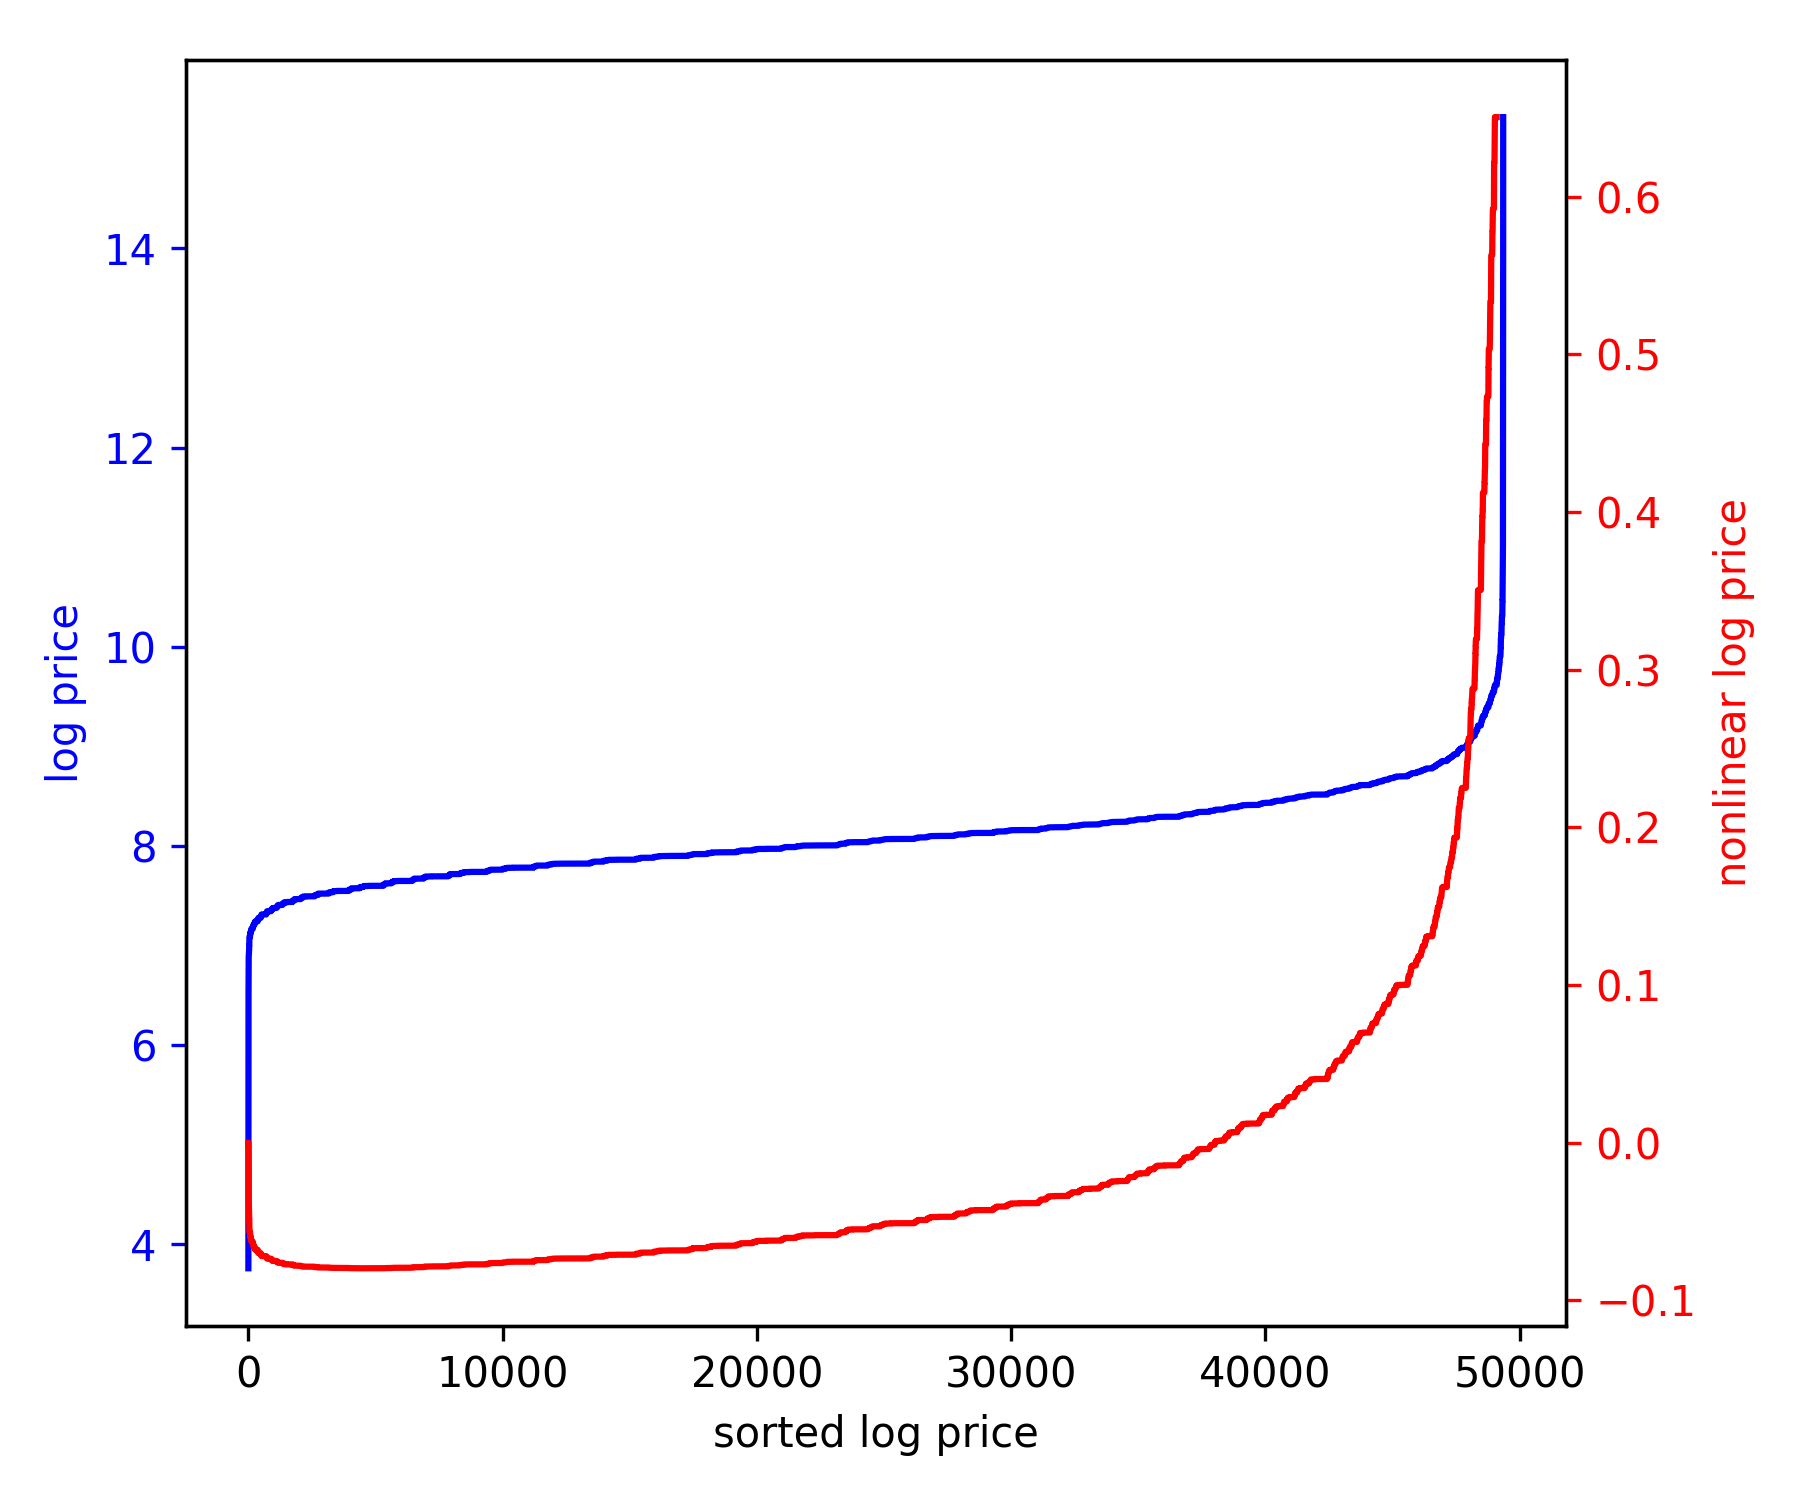
\includegraphics[width=0.33\textwidth]{pic/nonlinear_price.png}
}
\caption{The Non-linear Transformation on Price data}\label{nlprice}
\end{figure}

\subsection{Human Factor - The Manager}

~~~~ According to RentHop's ranking algorithm HopScore, listing quality, listing manager performance, and listing freshness will decide what kinds of listings will be more visible than others. Therefore, listing manager has an important contribution to the popularity of the listings. We measure the performance of every listing manager by the engineered feature ``manager\_skill''. 

We qualify the performance of mangers, which is defined by the ratios of apartments in each interest-level, under his/her management, and an overall score of the manager is computed based on the three ratios.
\begin{align*}
& \text{high\_rate} = \frac{\text{listings of high-interest}}{\text{total listings under his management}} \\
&~~~~~~~~~~~~~~~\text{(similar for medium\_rate and low\_rate)}\\
& \text{manager\_skill} = 2\times\text{high\_rate} + \text{medium\_rate}
\end{align*}
 And only the managers with at least 20 historic listings will be taken into evaluation (we do not compute the ratios and overall score for managers with not enough experiences). For the missing values, we use the mean rate/score of the evaluated managers. This set of features is an alternative to categorical manager ID number.

An overview of manager performance is shown in Figure \ref{mngr_skill}.
\begin{figure}[htbp]
\centering
    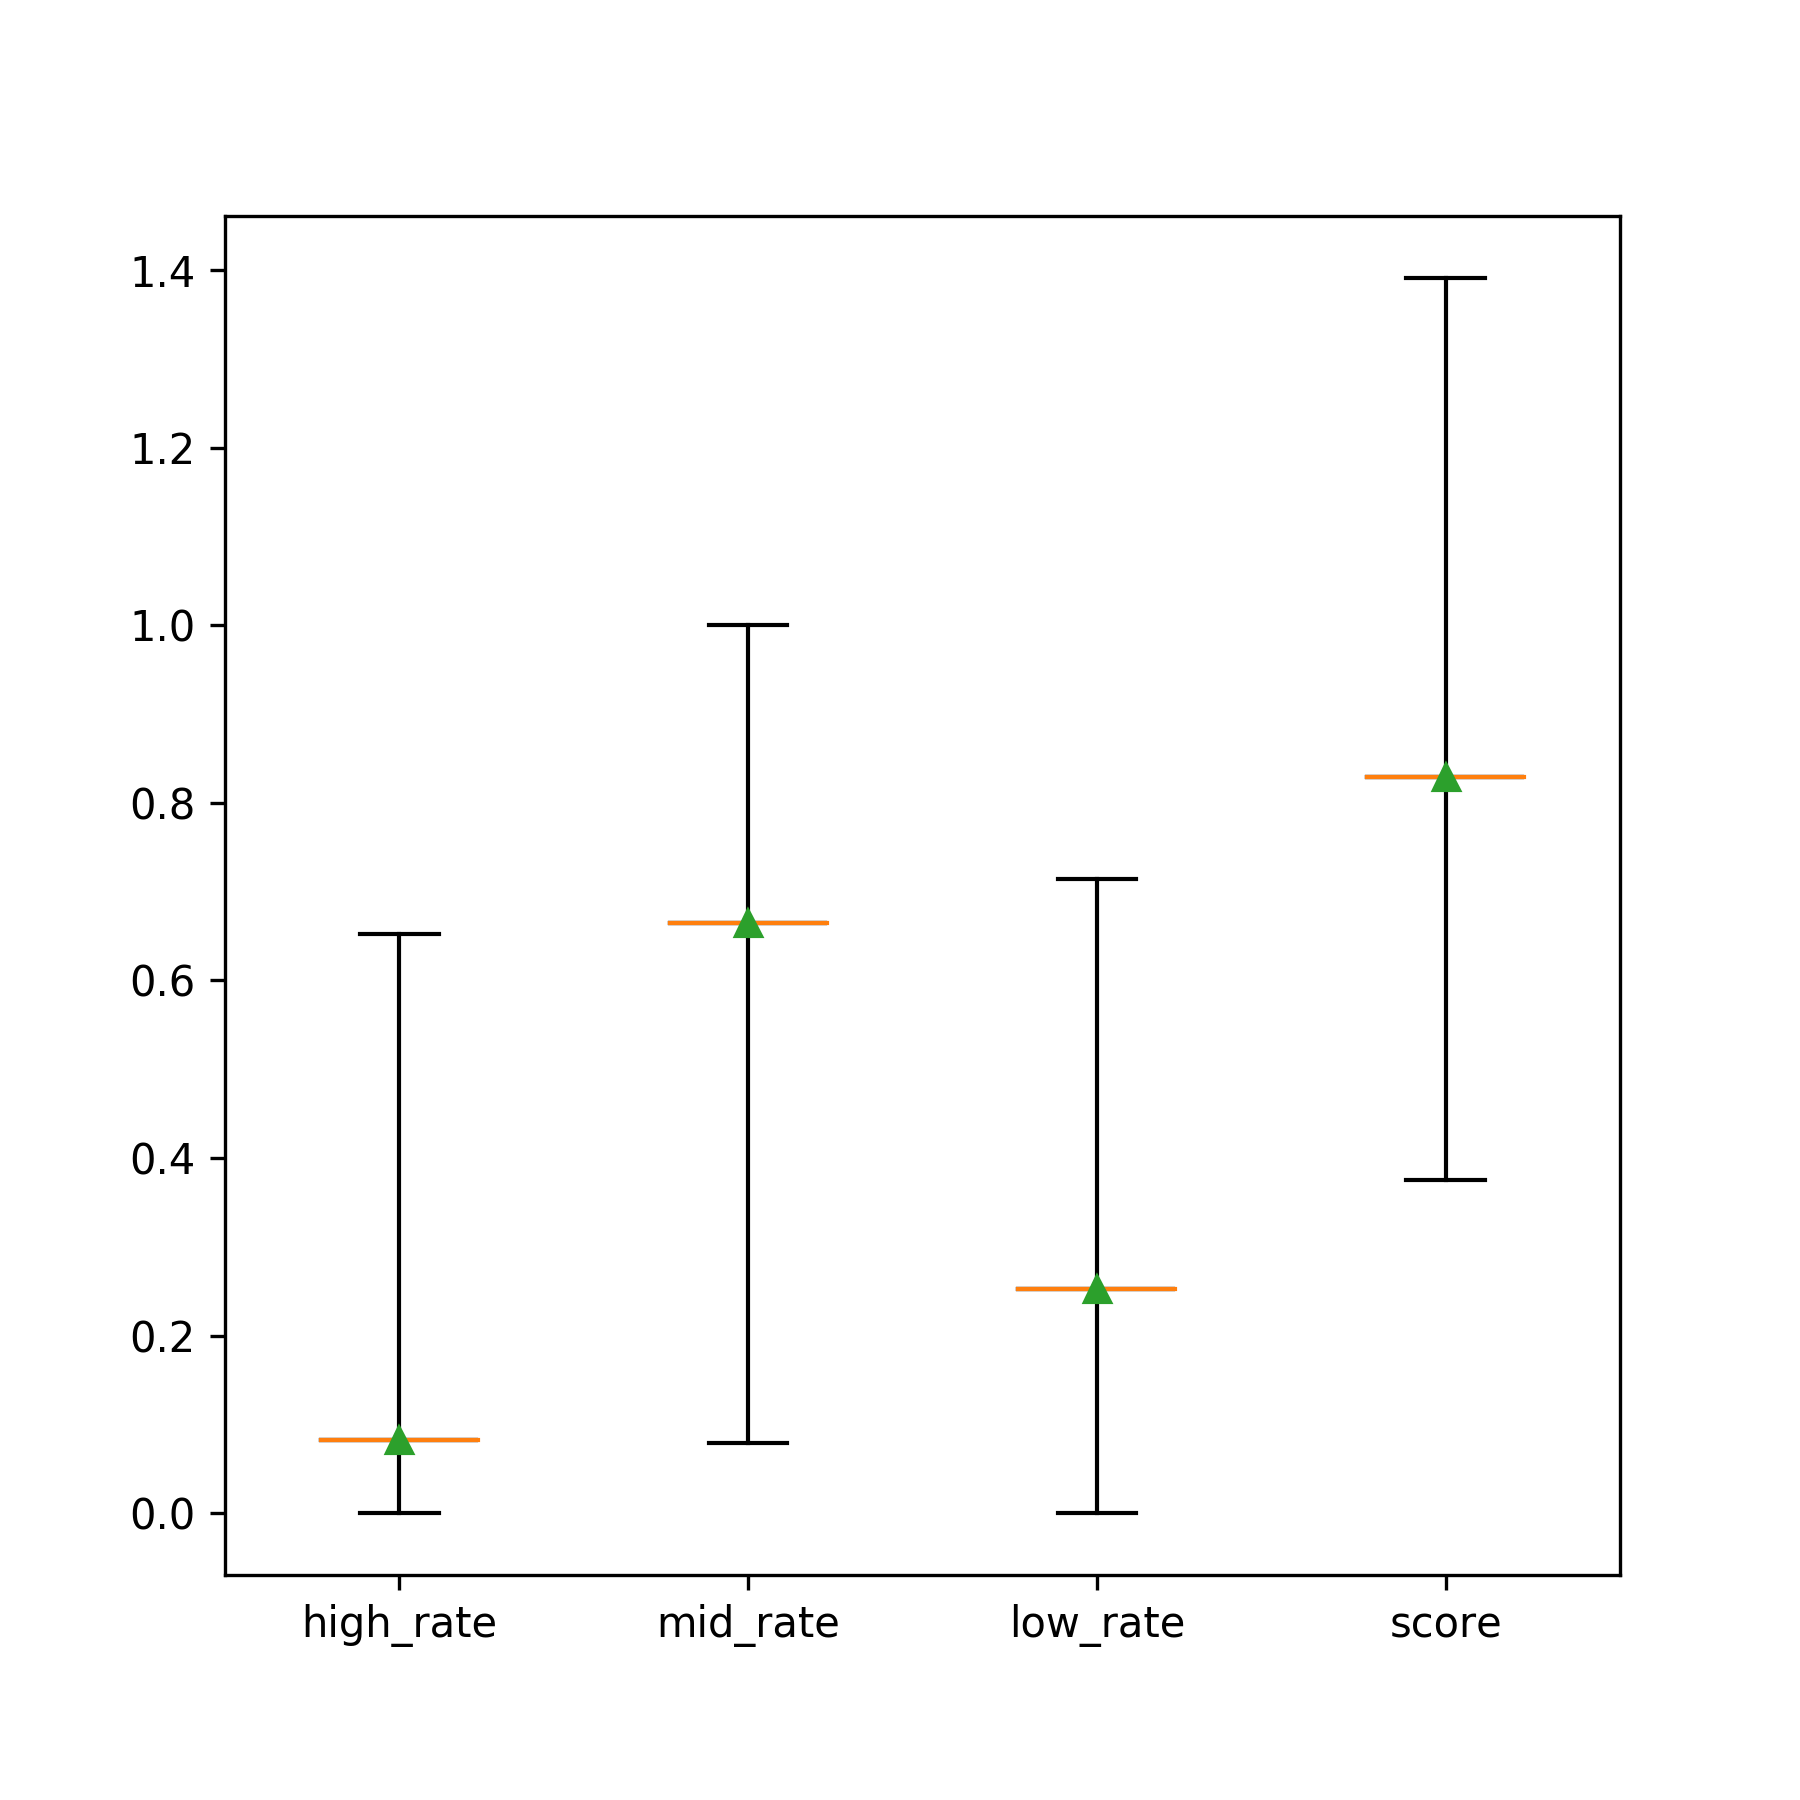
\includegraphics[scale=0.4]{pic/manager_skill.png} 
    \caption{Performance of listing managers in the Training set} \label{mngr_skill}
\end{figure}

\subsection{Clustering on Geographical Data}

~~~~ Given longitude and latitude, we found that most listings are in NY metropolitan area. 
we can try grouping the listings into clusters of in New York plus one extra category for outside NY. While longitude and latitude can present accurate location, it's hard to compare nearby listings. Either we need a distance metric for every two listing, or can we make them into small clusters. We tried clustering the data into 50, 100, 500, and 1000 clusters and compare the in cluster median price with training set median. We hope that the differences can show the influence of geographical location. Furthermore, we compare the in cluster median price of different types of bedroom-bathroom combinations for a more accurate result. 

Because cluster is also a categorical features, we tried the same transformation for all the categorical features and compare the performance of each transformation.
\begin{figure}[htbp]
\centering
    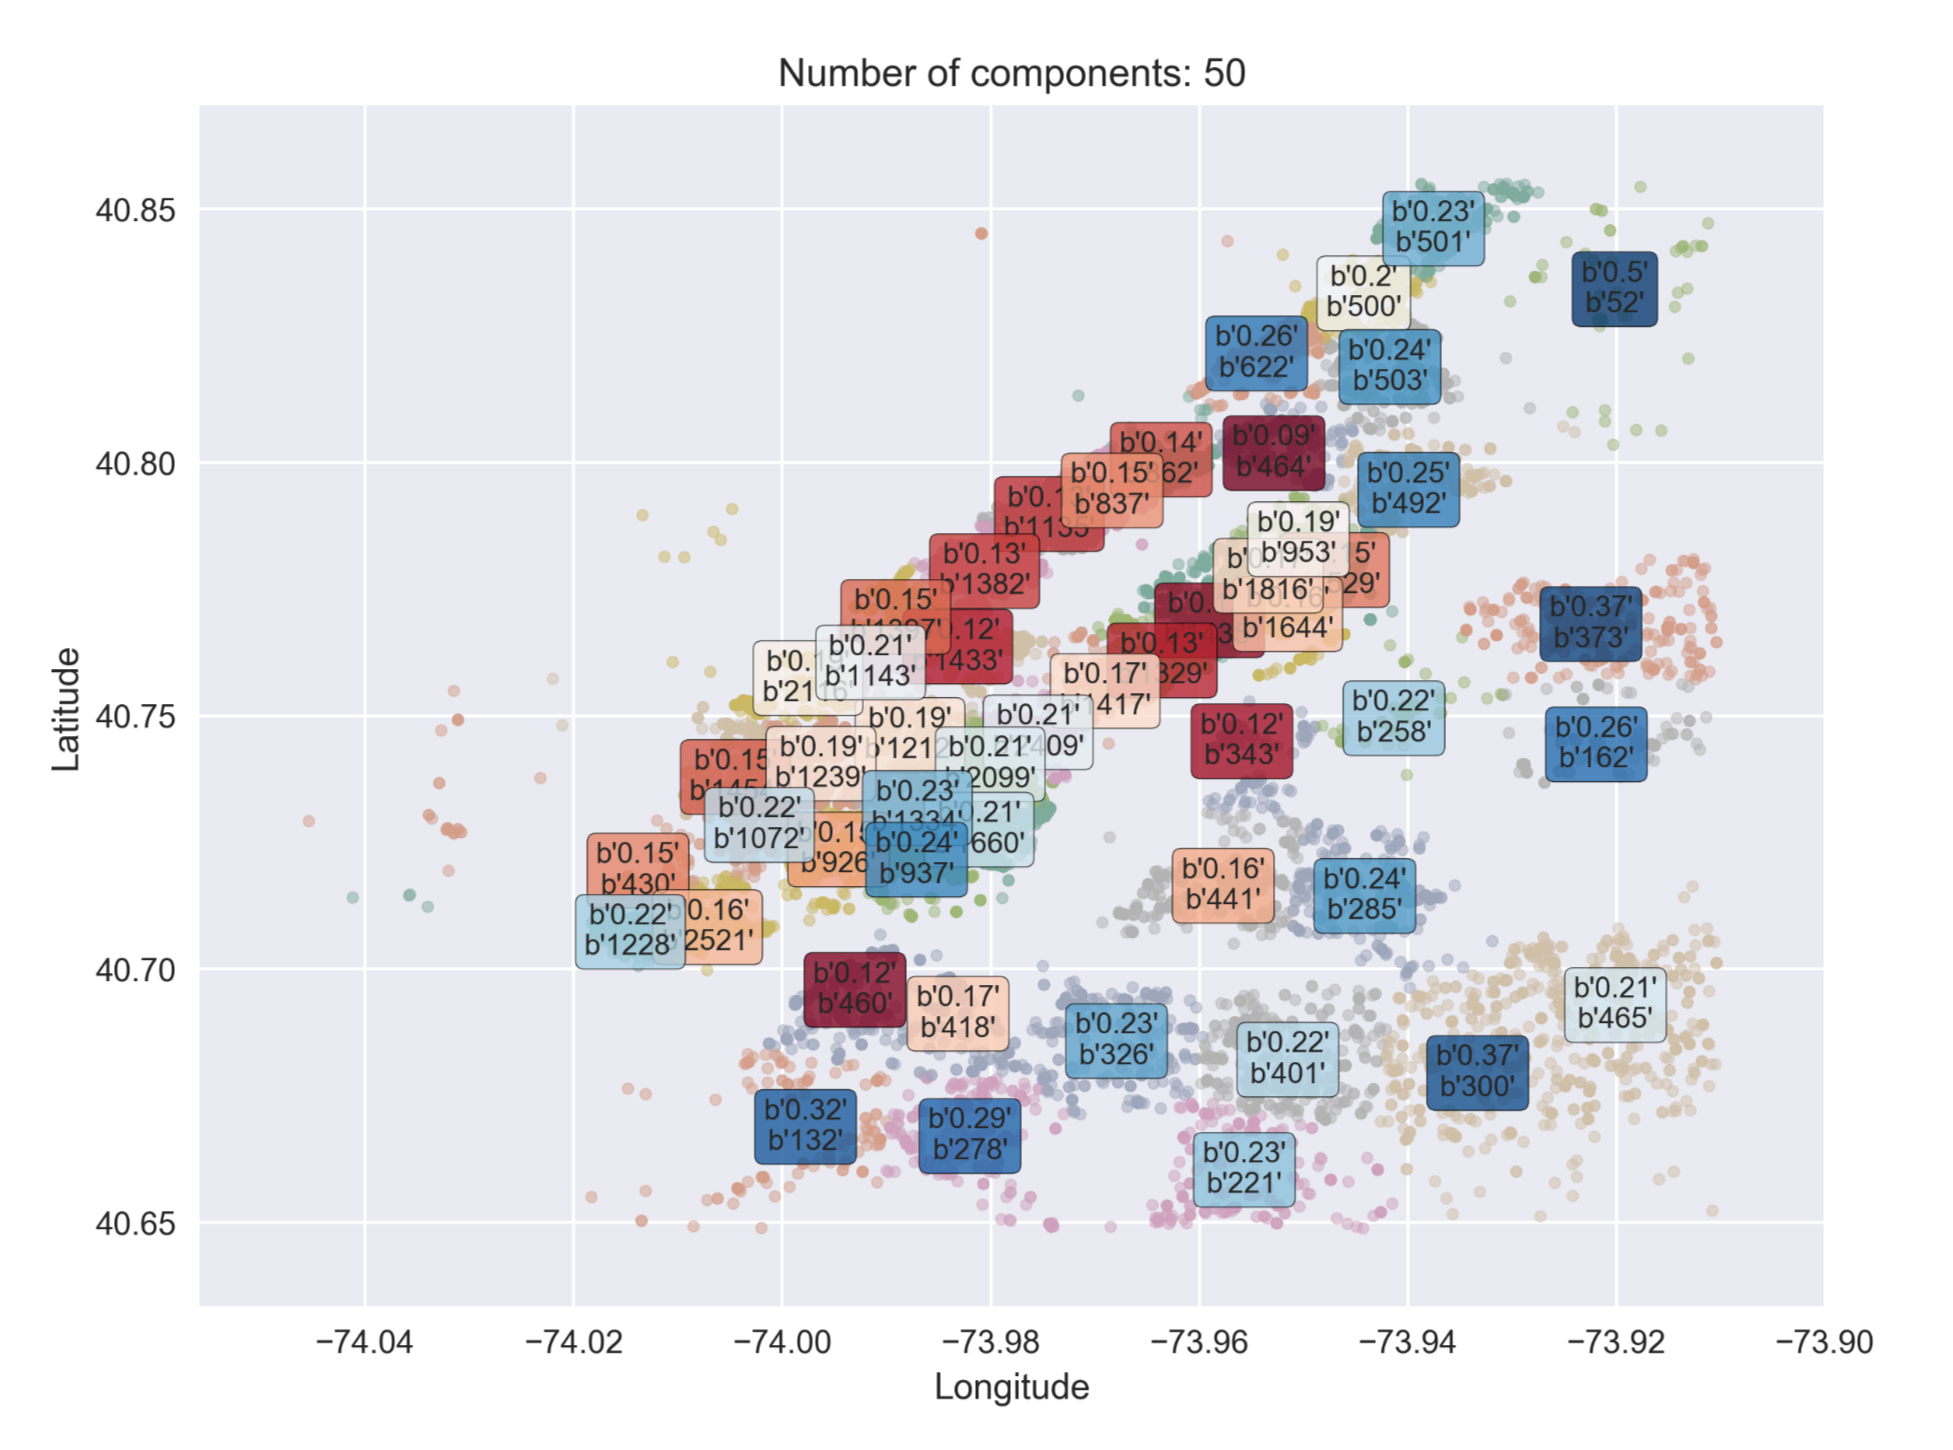
\includegraphics[scale=0.16]{pic/cluster_50.png} 
    \caption{An example with 50 clusters on location data} \label{cluster50}
\end{figure}

\subsection{Processing the Description and Vocabulary Features}

~~~~ The first step of processing vocabulary data, including two fields -``features'' and ``description'', is to remove synonyms, as the descriptions in the listings are entered by different managers/officers. 

With observation from the training data, we can see that different expressions of similar meaning are employed in the descriptions. For example:
\begin{align*}
    & \text{\textbf{24-hour \& 7-day services}: 24, 24/7, 24-7, ...} \\
    & \text{\textbf{fitness}: fitness room, fitness space, gym, ...} \\
    & \text{\textbf{air-conditioning}: ac, a-conditioner, Air-Con, ...}
\end{align*}

The removal of synonyms is implemented with 3 steps, clean, merge and replace. The second step is realized by only looking at the first 4 (or 5) characters of the words, and the vocabularies with identical first 4 characters will be replaced (in the next step) by an identical word. By removing the synonyms in the descriptions, the number of unique words is reduced, which benefit the processing of count-vectorization.
 
Hence, after the cleaning of ``features'' and ``description'',  we obtain sparse features of tf-idf information through word-map vectorization. Regularization is introduced to avoid overfitting.

%---------------------------------------------------------------- 5. Results
\section{Results} \label{results}

\subsection{Performance of Different Models and Feature Sets}

~~~~Different combinations of features are tested. Starting with our base model with only 5 features: \{`bathrooms', `bedrooms', `latitude', `longitude', `price'\}, we add numerical features, categorical features, manager skills, non-linear price, and NLP features each round and sees a steady decrease in log loss. We see a significant performance boost using Random Forest (0.6) and XGBoost(0.54) over logistic regression (0.75). 

In our model selection process, we see a stable relative performance among different feature sets. After repeated testing, we conclude that the set of features including numerical features (original and added), categorical features, non-linear price, manager scores and the tf-idf features (150-200 vocabularies) gives the overall best performance, with gradient boosting methods. %The enormous tf-idf features are not plotted in the figure of feature importance.

Using XGBoost as our training algorithm, we compare the result using different transformations of categorical data. We see an average 0.005 performance lead using the categorical features as numerical values over their transformations. This is also true for random forest. It seems that it?s okay to regard categorical data as numerical data when using tree based methods. 

We also tried substituting longitude and latitude with clusters of 500. We see a performance loss about 0.014. Since we use longitude and latitude to do clustering, part of information is lost during the process. When we try including cluster median difference as a new feature, we get a significant boost to 0.52 of the test log loss. However, we found that the model overfits quickly as during the training process, optimum depth of tree reduced from 7 to 3, a 16X shrink in numbers of  tree nodes. This indicates that the price difference to nearby similar listing could be a great feature, but only if we get it right and unbiased. We tested the feature with extra data available on Kaggle and the result is 0.66, which is not consistent with our local testing result. So we didn?t include this feature in our final version.

\begin{figure}[h]
\centering
\subfigure[Progress with feature sets]{
	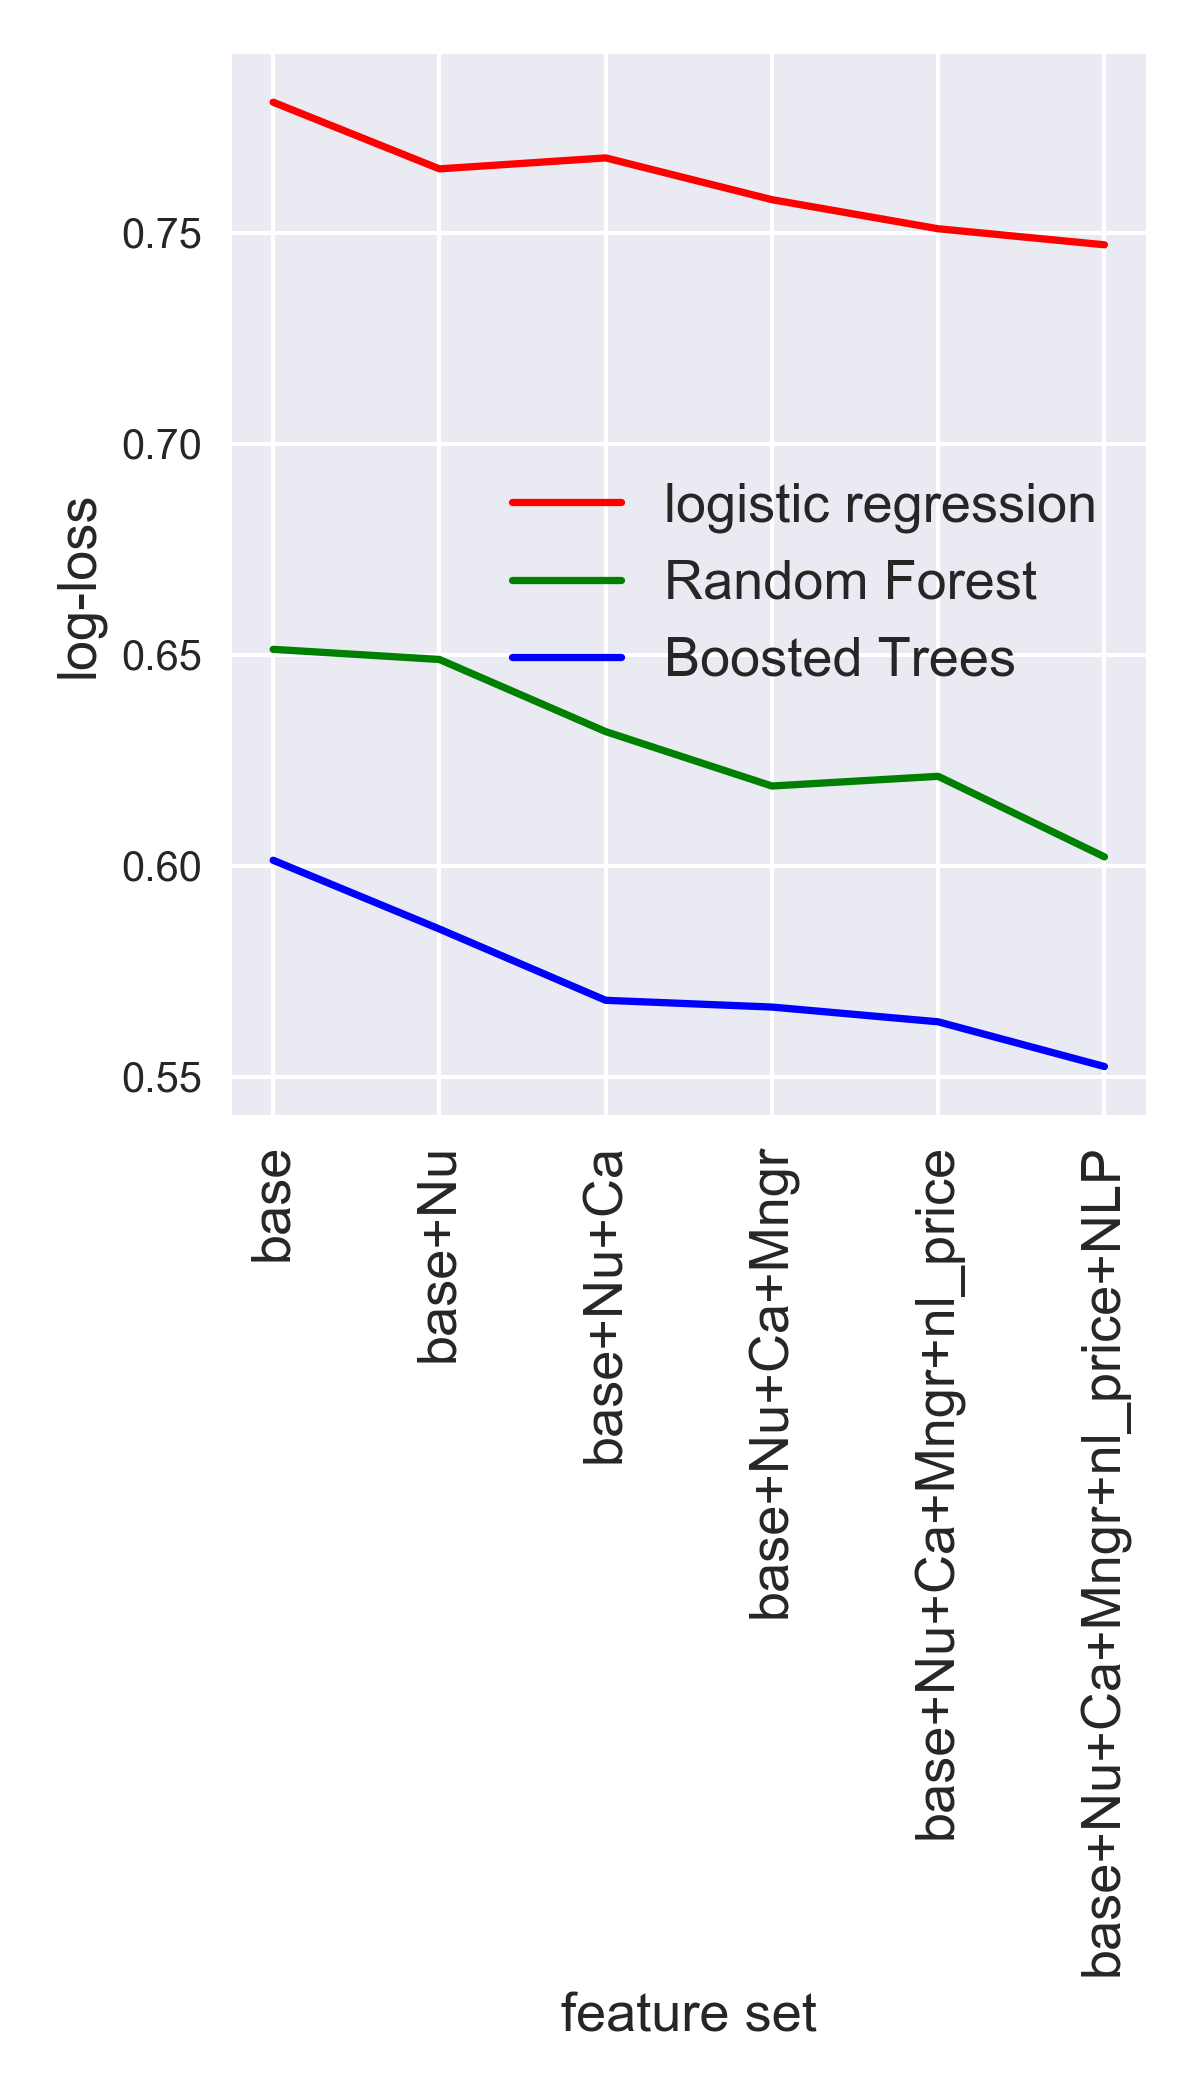
\includegraphics[width=0.25\textwidth]{pic/loss_improve.png}
}
\subfigure[Performance of algorithms with best feature set]{
	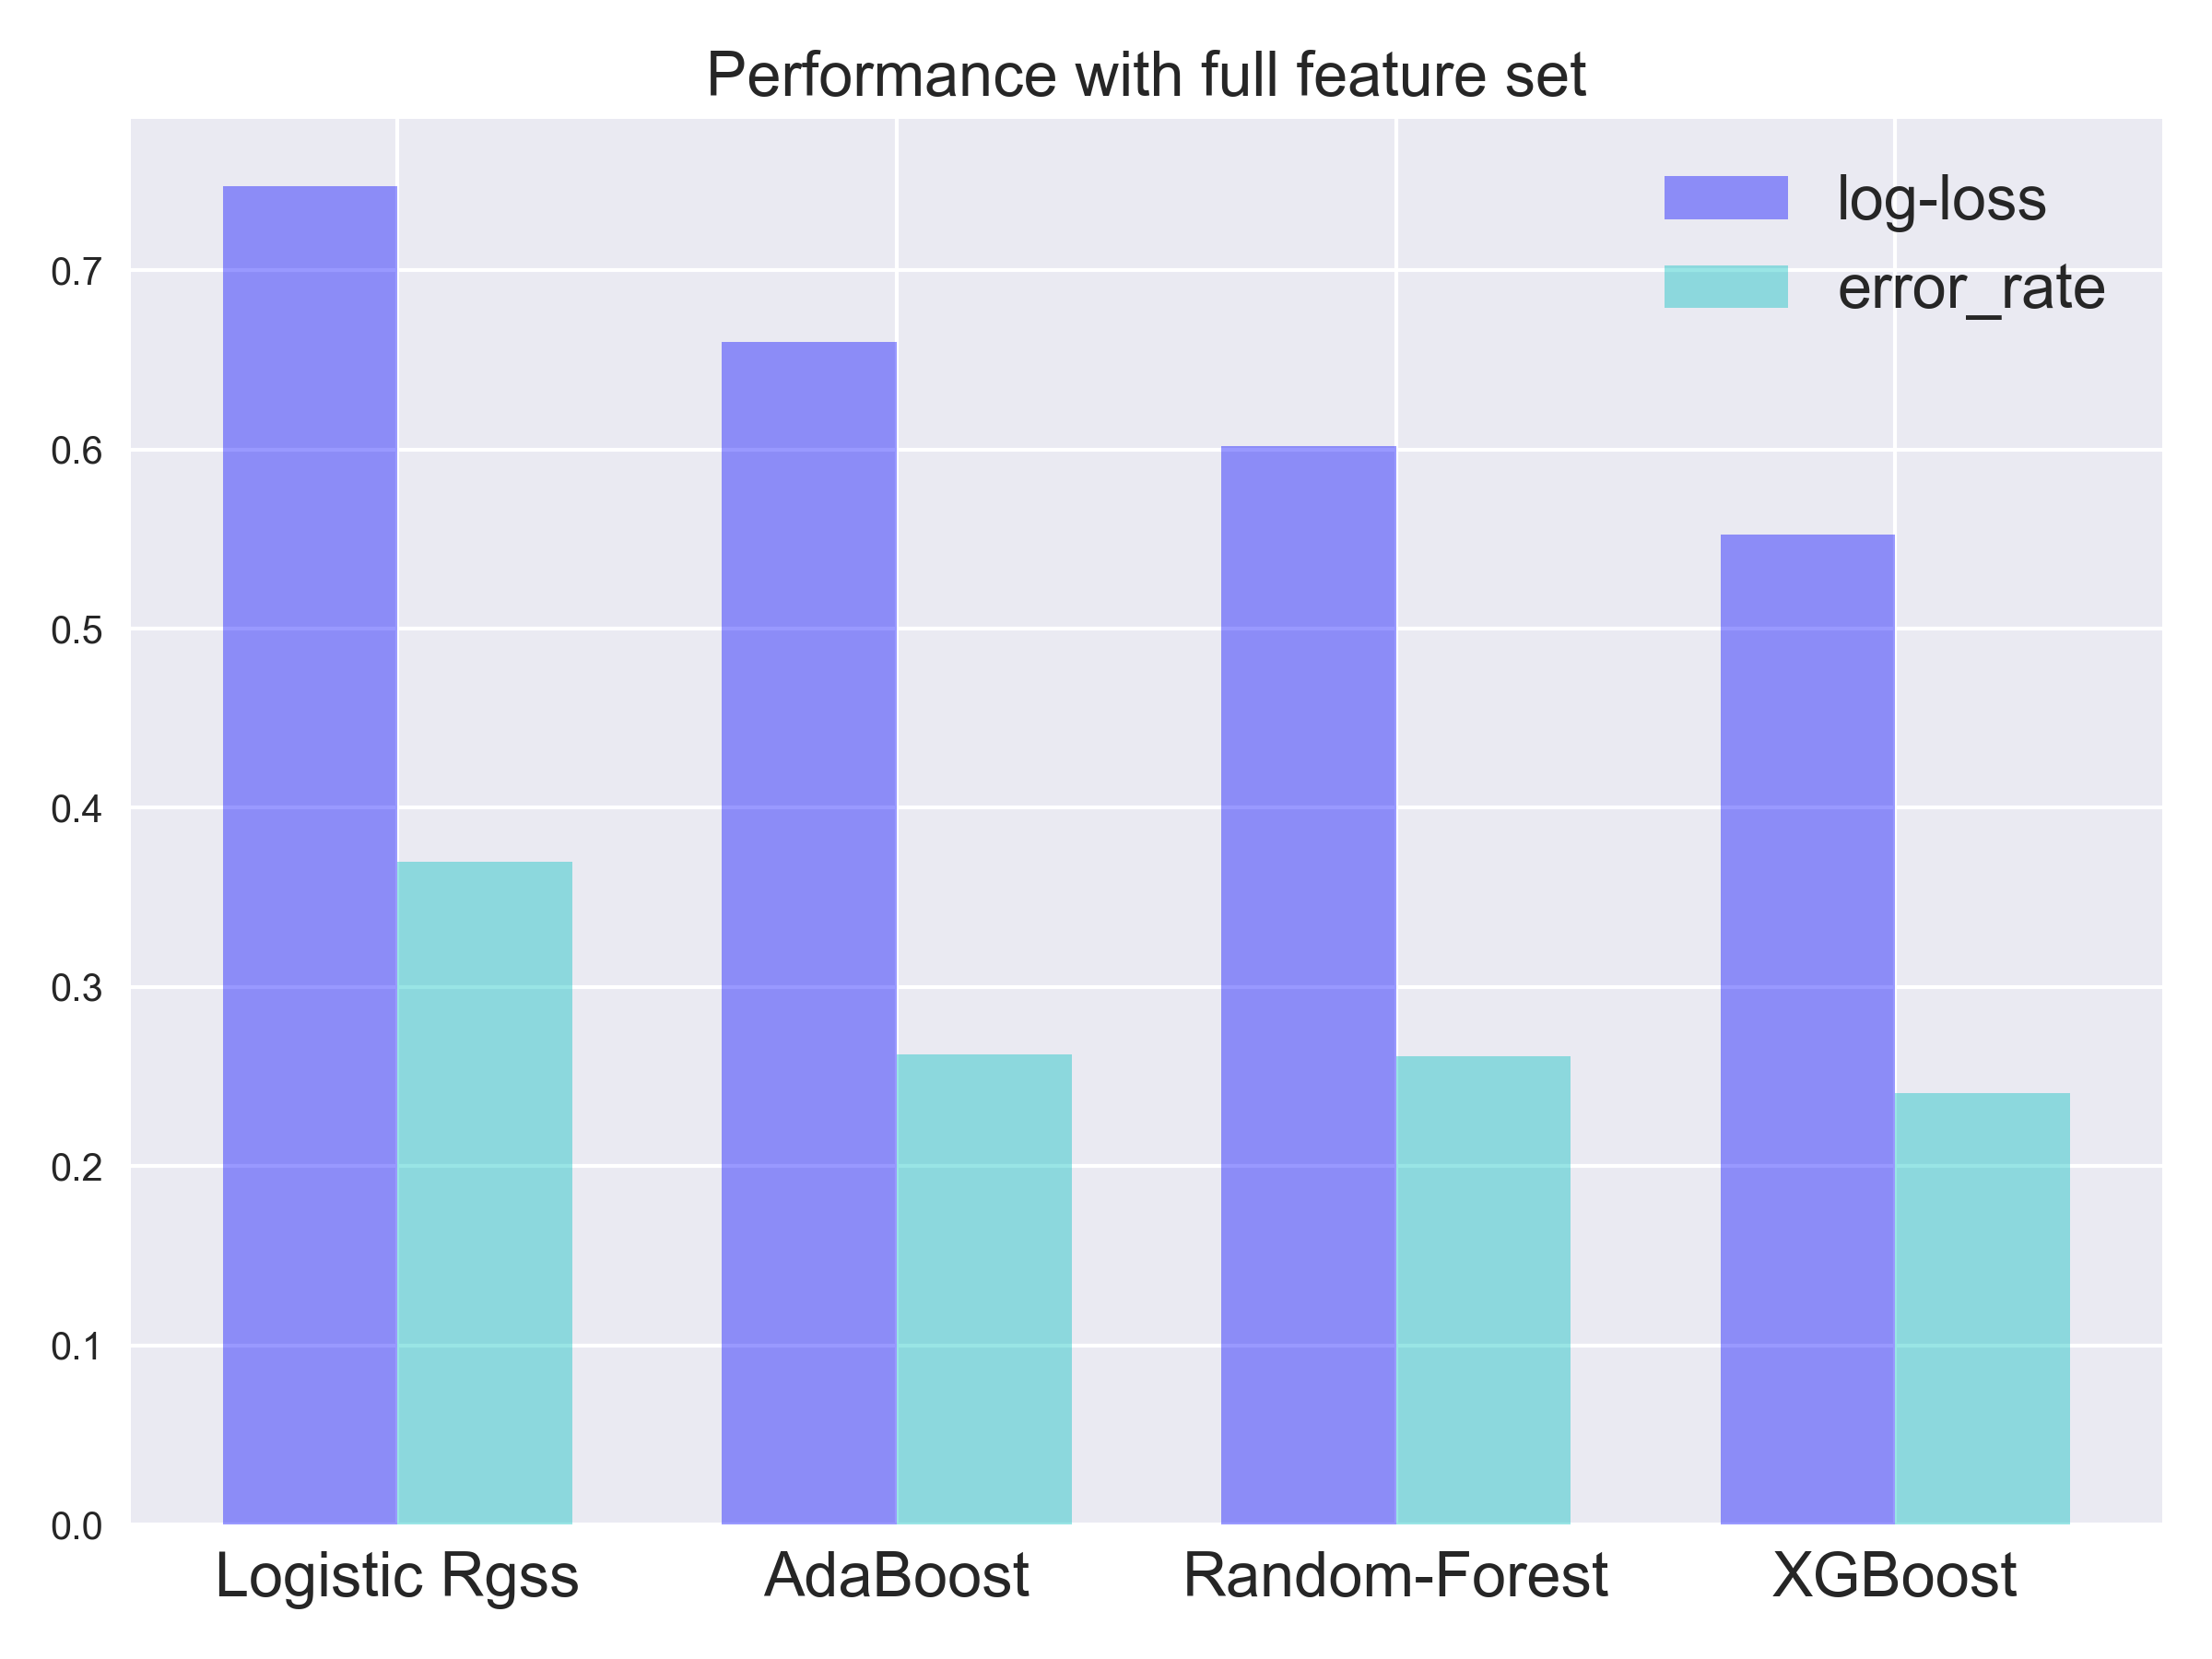
\includegraphics[width=0.62\textwidth]{pic/compare_result.png}
}
\caption{Progress and Comparison of different algorithms}
\label{comp_result}
\end{figure}

\subsection{The Roles of Features}

~~~~ Ranking by splitting entropy minimizing rule, we list most important features in Figure \ref{ft_importance}. We can see that the manager, location, price drive the interests from customers. 

As we can see from Figure \ref{ft_importance} (a), the manager plays an important role in the interest-level of listings. People are looking at the average performance of the listing manager, and the information provided by the manager also counts for the result. Managers who writes explicit descriptions of apartments are more likely to attract customers. 

Besides, from (a) to (b) in Figure \ref{ft_importance}, the categorical \texttt{manager\_id} is replaced by the features of \{`high\_frac', `medium\_frac', `low\_frac', `manager\_skill'\}, evaluated from the historical performance of listing managers. By breaking down the influence of listing managers, the total importance of this subset features related to managers is higher than that of \texttt{manager\_id} in the previous feature set. It also leads to an improvement of predicting the interest-level of listings. 

Similarly, the combination of \texttt{price} and \texttt{non-linear price} explains more about the result (or class, or interest-level) than single price information. 

The enormous tf-idf features are not plotted in the figure of feature importance. Top vocabularies includes: \{ `public\_outdoor', `laundry\_in\_building', `recreation\_facilities',  `eat', `24'(24/7 services), `no\_fee', `air\_conditioning', `private\_parking', `walls\_of\_windows', `pool', ...\}. Nothing surprising at all, considerations of facilities and community services always come first.

A seemingly abnormal fact is that \texttt{listing\_id} ranks high in the feature importance list. One possible reason, which comes from comparing (a) and (b) in Figure \ref{ft_importance}, is that listing managers tend to post clients' listing together. So listing ID will reflect impact of managers. Another conjecture is that, since the data contains high label-noise (the apartments receives different interests even if the room structures, facilities, and locations are the same), as we are using tree-based methods and looking for a splitter to reduce impurity, the only feature that we can rely on is the \texttt{listing\_id}, which is unique for each listing. 

\begin{figure}[h]
\centering
\subfigure[Basic feature with additional numerical and categorical features]{
	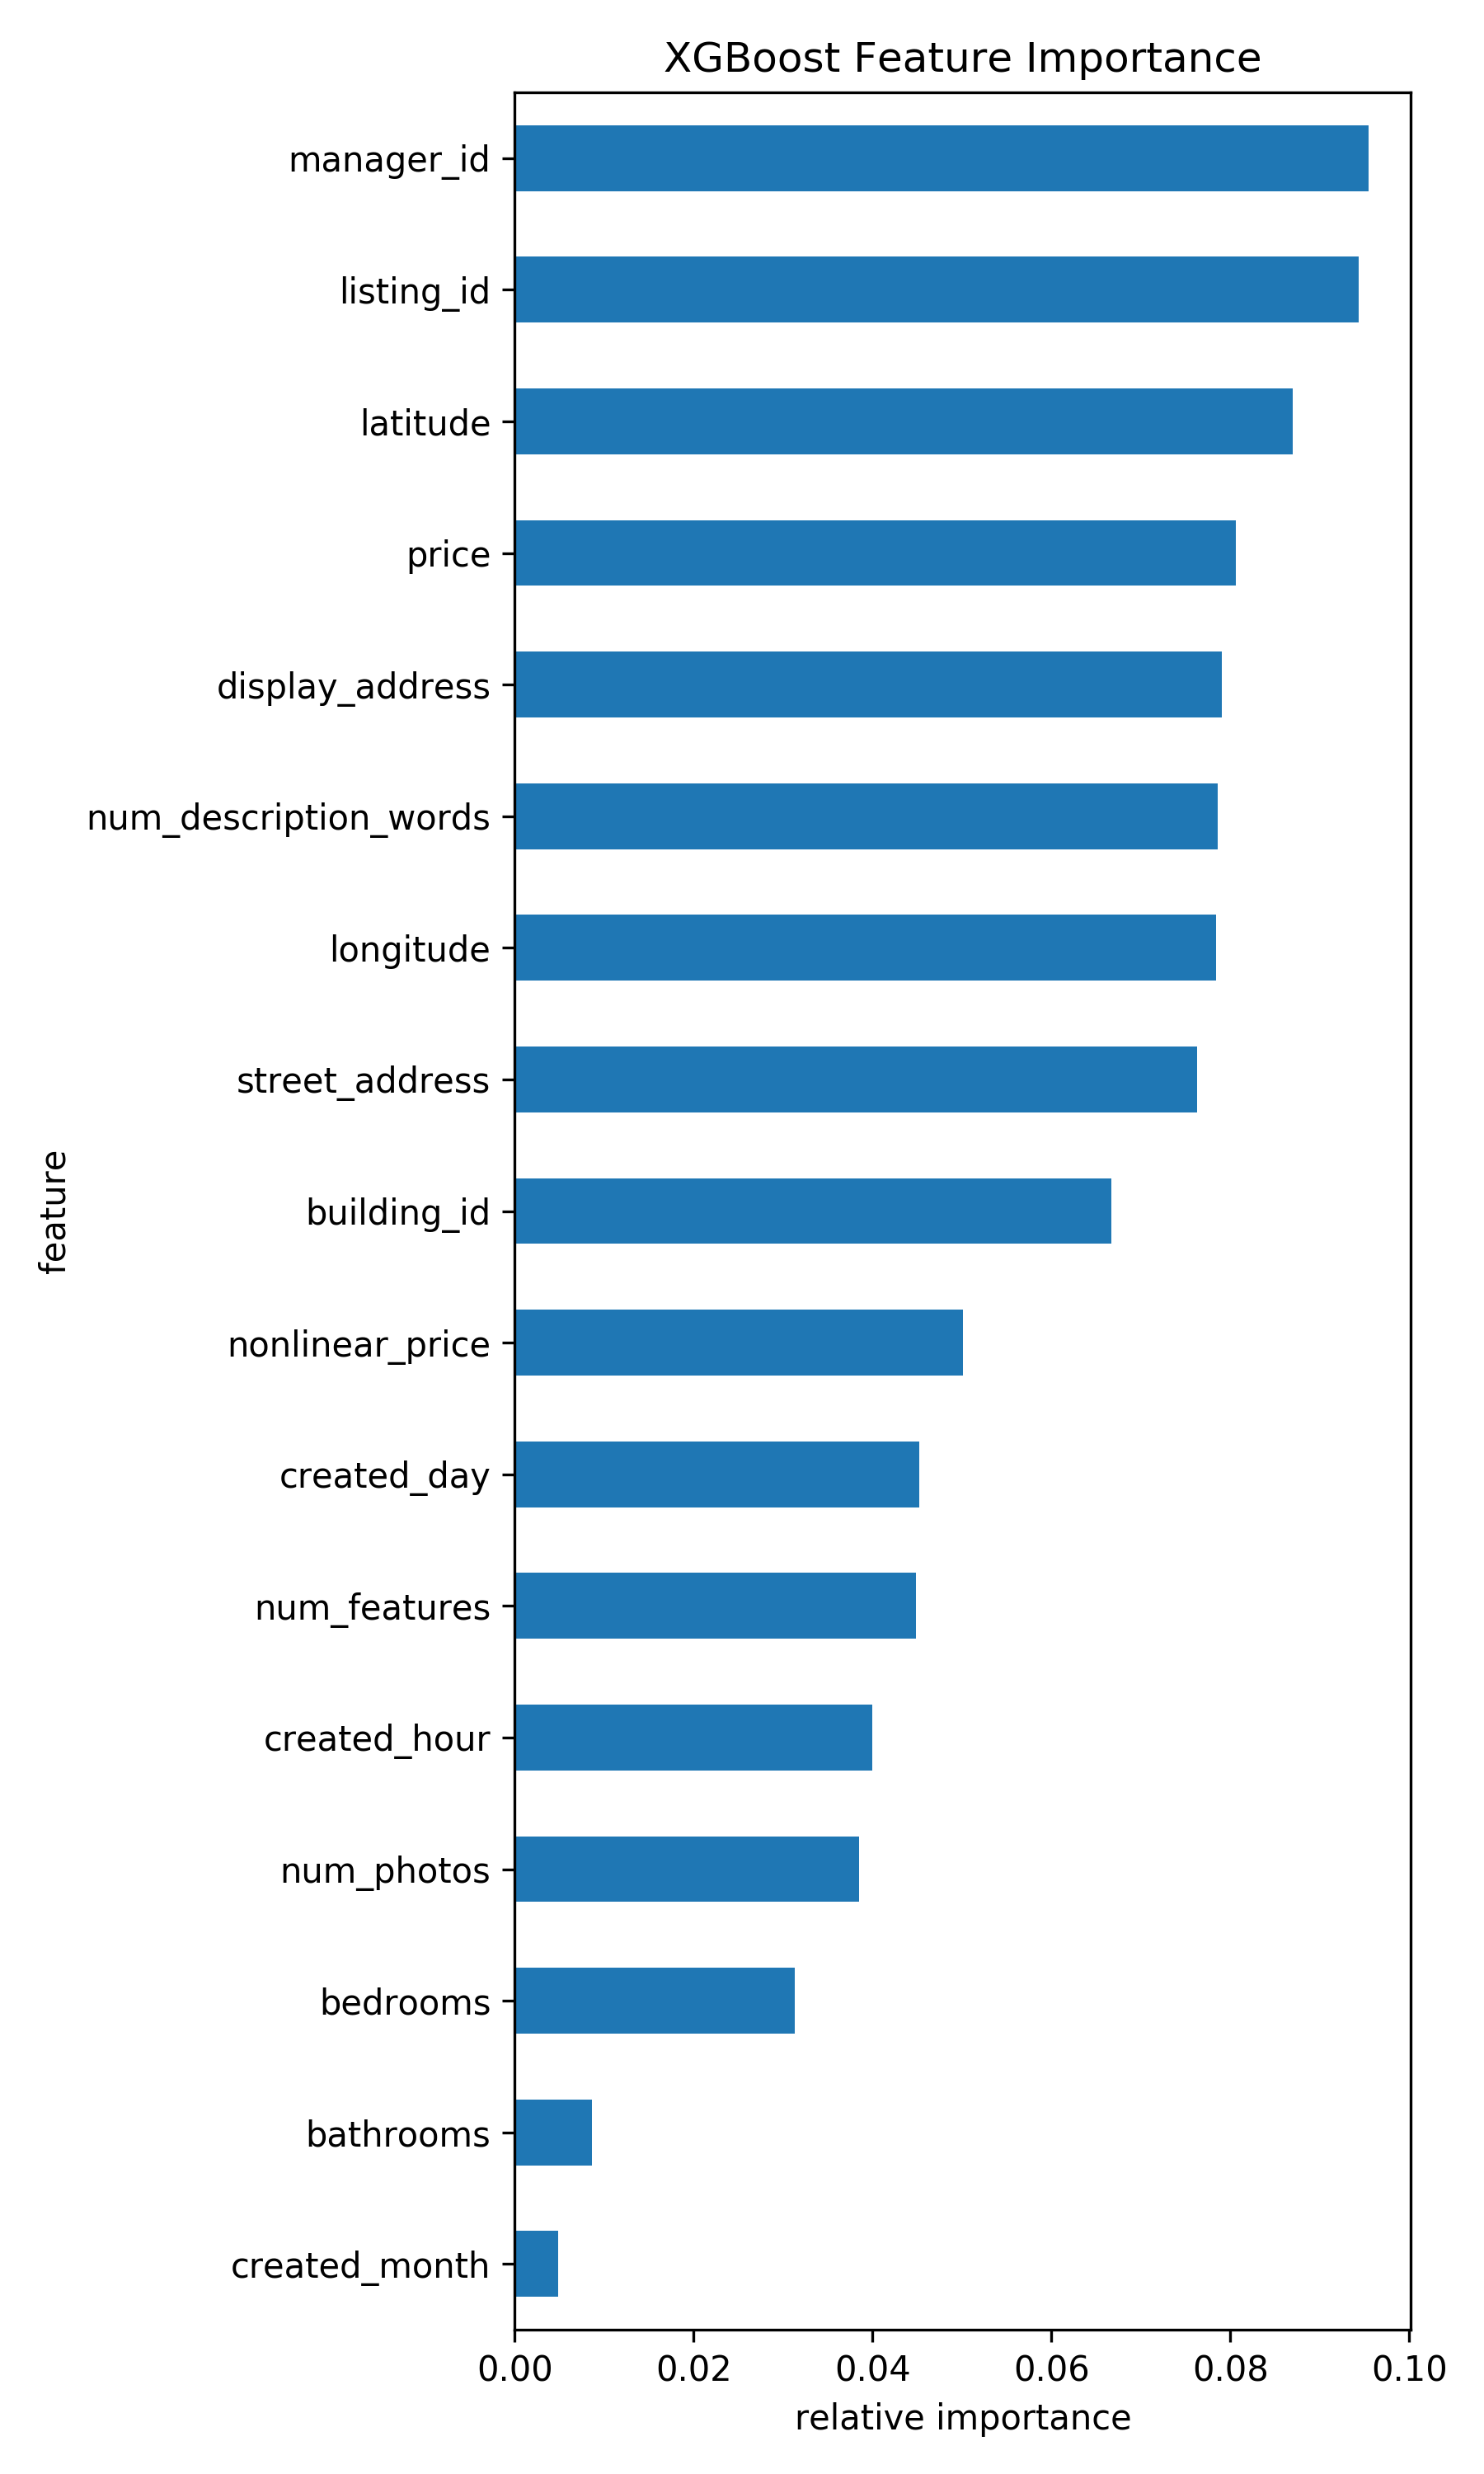
\includegraphics[width=0.45\textwidth]{pic/feature_importance_xgb_0.png}
}
\subfigure[Replaced manager\_id with manager\_skill]{
	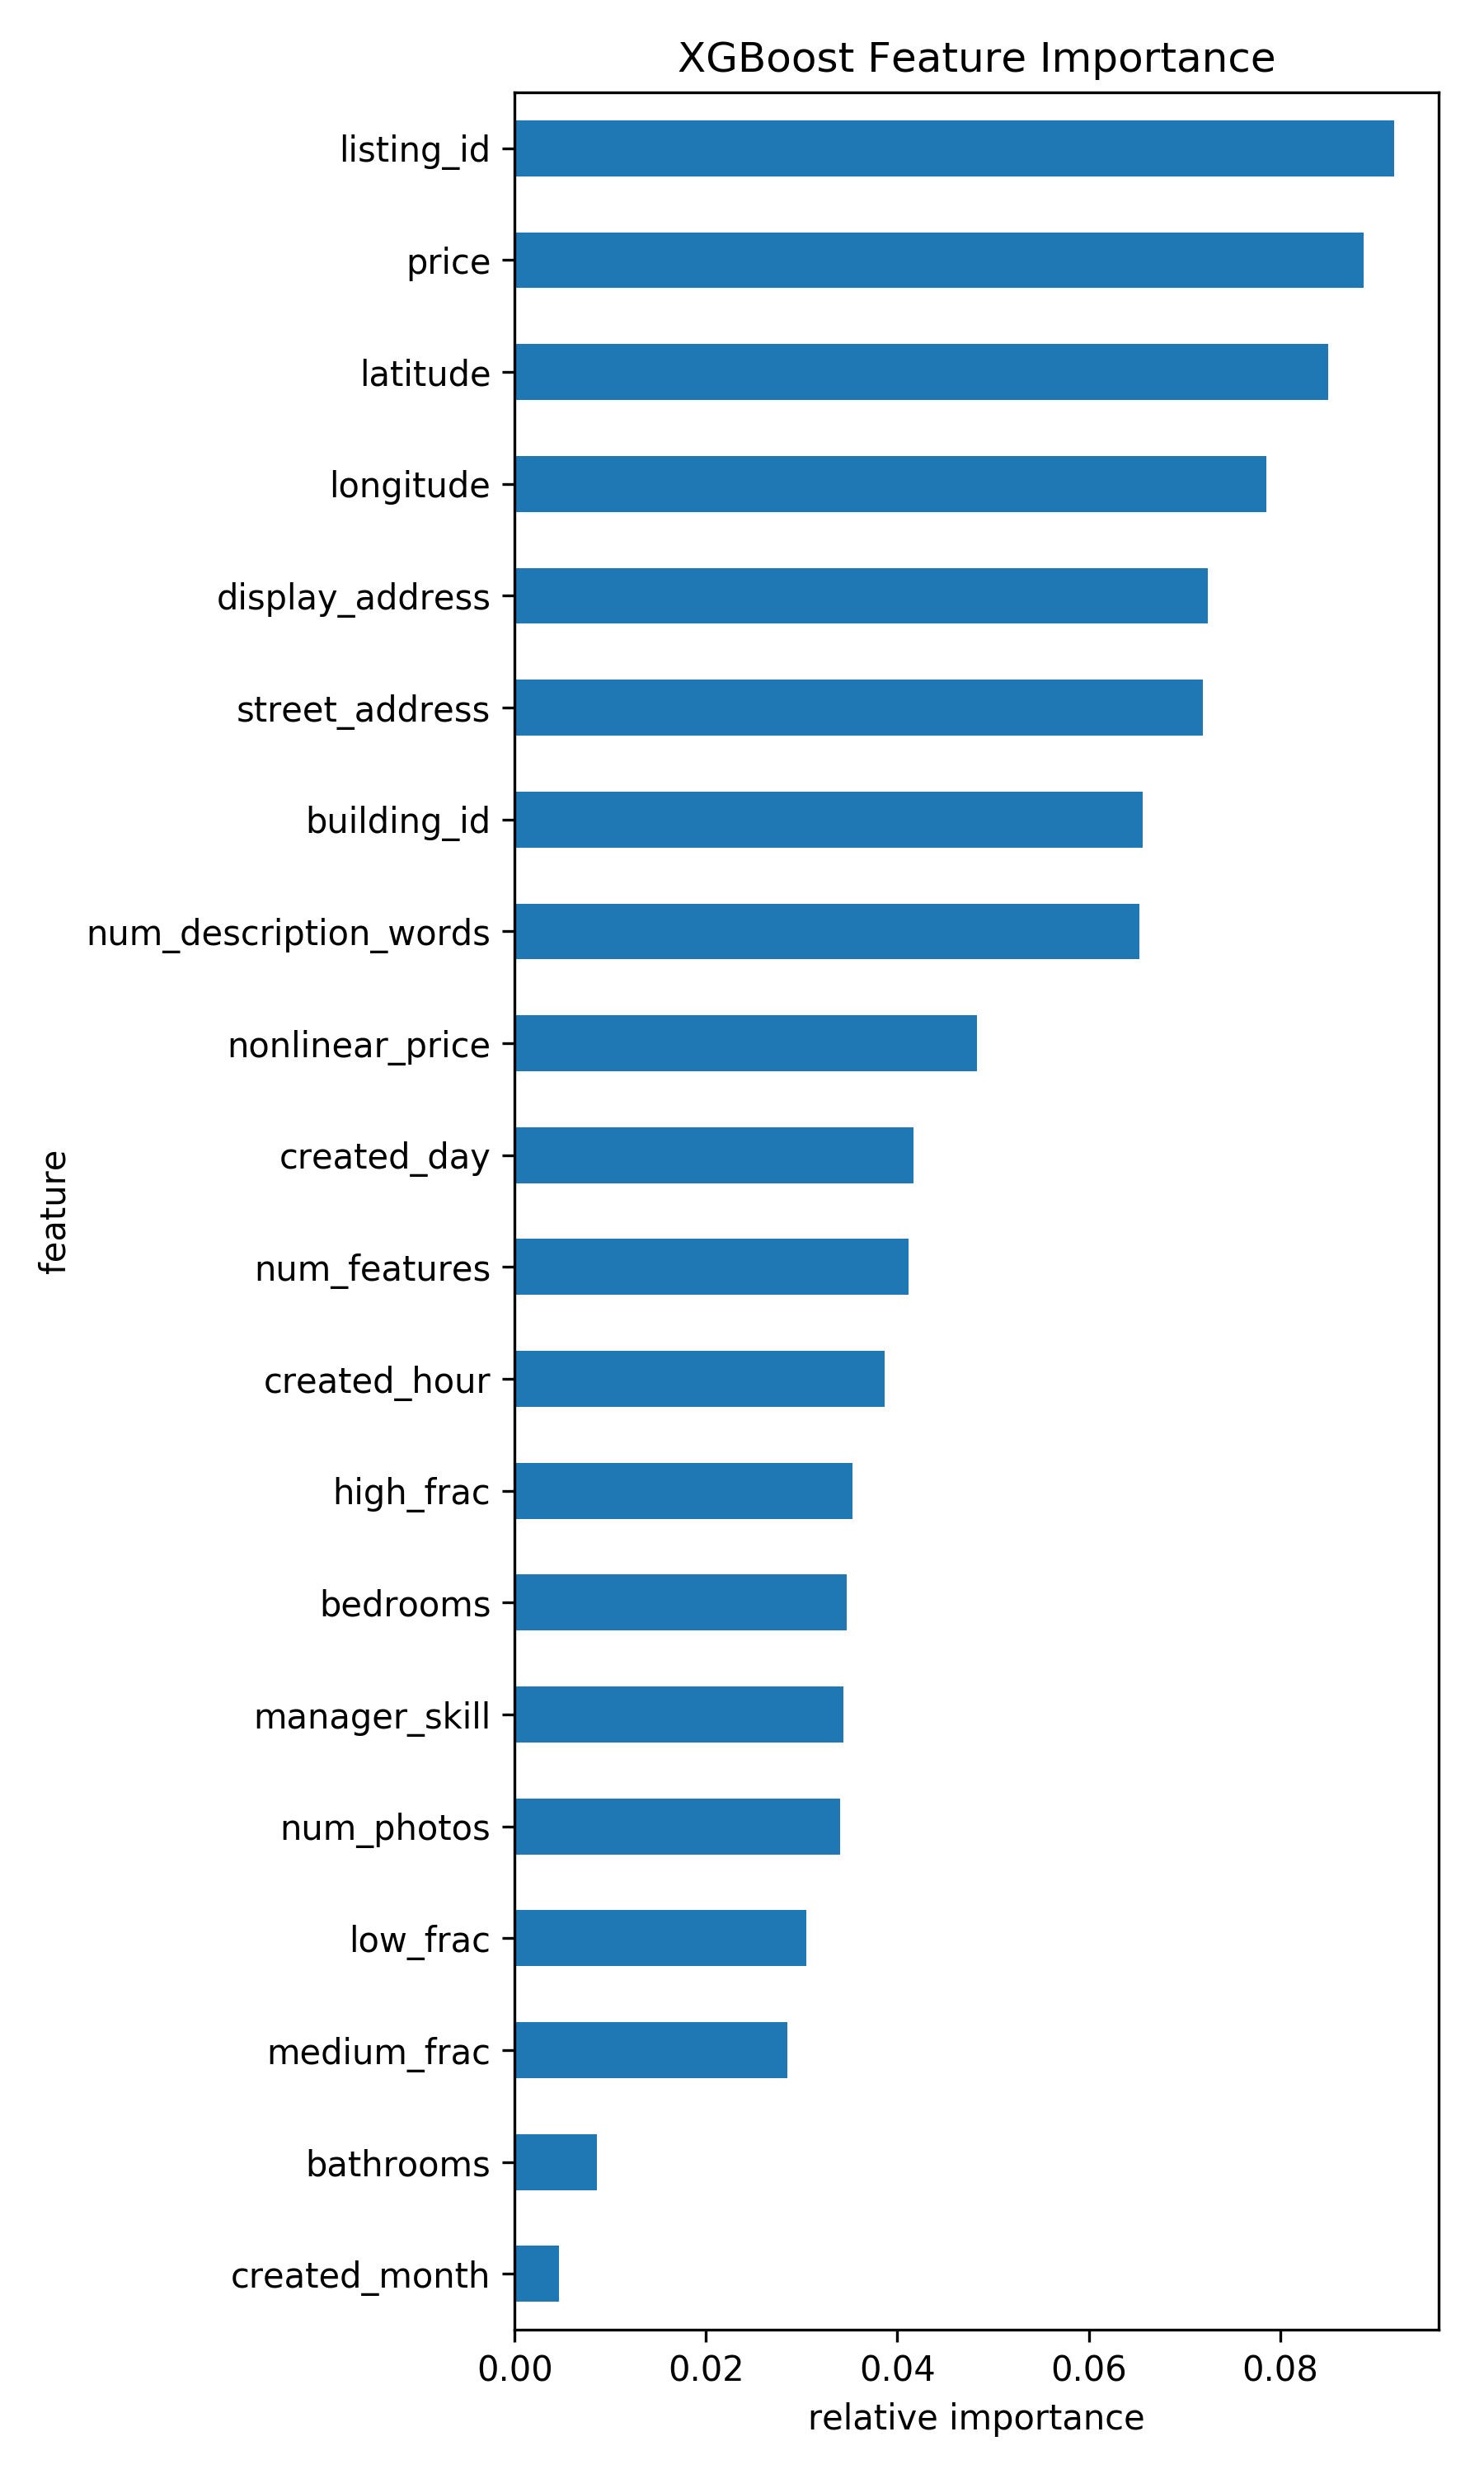
\includegraphics[width=0.45\textwidth]{pic/feature_importance_xgb_1.png}
}
\caption{Feature Importance with XGBoost}
\label{ft_importance}
\end{figure}
    

%------------------------------------------------------------- 5. Next Steps
\section{Next Steps} \label{nextsteps}

~~~~ There are photos on the website for most of the listings, which provides additional high dimensional Data. We can extract features like exposure, contrast in the photos. Neural Networks will be a good candidate to learn from the image features. Yelp has an application of convolutional neural network to find out beautiful photos among the photos submitted by reviewers. Given such a tool, we can add new features like how well the photos are shoot. Also, using neural network can help us find whether the photos are real, and whether the lister provides floor plan \cite{yelp}. However, without proper labeling, we can't do supervised learning of these features. % REF: Finding Beautiful Yelp Photos Using Deep Learning

Information about the convenience of transportation is missing in this dataset, though partly revealed in the descriptions. A combination with urban transportation system and medical systems (i.e. distance to the nearest train station or clinic) might be good to help.


%----------------------------------------------------------- 7. References
\begin{thebibliography}{9} 

\bibitem[1] Friedman, Jerome, Trevor Hastie, and Robert Tibshirani, \emph{Additive logistic regression: a statistical view of boosting (with discussion and a rejoinder by the authors).} The Annals of Statistics 28.2 (2000): 337-407.

\bibitem[2] Niculescu-Mizil, Alexandru, and Rich Caruana, \emph{Obtaining Calibrated Probabilities from Boosting.} UAI. 2005.

\bibitem[3] Niculescu-Mizil, Alexandru, and Rich Caruana, \emph{Predicting good probabilities with supervised learning.} International Conference on Machine Learning. ACM, 2005.

\bibitem[4] Van Smeden, Maarten, et Al, \emph{No rationale for 1 variable per 10 events criterion for binary logistic regression analysis.}, BMC Medical Research Methodology 16.1 (2016): 163.

\bibitem[5] Will McGinnis, \emph{Beyond One-Hot: Aa Exploration of Categorical Variables}, In {\em Will's Noise}, Nov 29th, 2015

\bibitem[6]{yelp} Alex M., \emph{Finding Beautiful Yelp Photos Using Deep Learning}, In Yelp Engineering Blog, Nov 26th, 2016

%\bibitem[1]{Doe} Gregory Connor, \emph{The Three Types of Factor Models: A Comparison of Their Explanatory Power}, Financial Analysts Journal, May/June 1995.
%\bibitem[2]{Ptfo} ``Portfolio'' \emph{Investopedia}, N.p., 25 Nov, 2003. Web. 
%\bibitem[3]{R_ex}``Excess Returns" \emph{Investopedia}, N.p., 06 May 2016. Web. 
%\bibitem[4]{bcts}``Backtesting" \emph{Investopedia}, N.p., 25 July 2015. Web.
%\bibitem[5]{Adr} Andrew Rudd and Henry K. Clasing, \emph{Modern Portfolio Theory: The Principles of Investment Management}, Orinda, CA, Andrew Rudd, 1988.
%\bibitem[6]{rcg} Richard C. Grinold and Ronald N. Kahn, \emph{Active Portfolio Man- agement: A Quantitative Approach for Producing Superior Returns and Controlling Risk}, Second Edition, McGraw-Hill Professional Publishing, Columbus, OH, 1999.
%\bibitem[7]{cross} Lee Chi-Wen Jevons, \emph{Stochastic Properties of Cross-Sectional Financial Data}, Journal of Accounting Research 23.1, 1985.
%\bibitem[8]{maxdd} Hamelink, F. and M. Hoesli, "The Maximum Drawdown as a Risk Measure: The Role of Real Estate in the Optimal Portfolio Revisited", working paper (June 24), 2003.
%\bibitem[9]{MPT} Harry Markowitz, \emph{Portfolio Selection}, The Journal of Finance, Vol. 7, No. 1, pp. 77-91 Mar., 1952. 
\end{thebibliography}


\end{document}
